In this section, we present the quantitative and qualitative outcomes of our experiments. We compare the baseline Stable Diffusion 3.5 Large Turbo (SD3.5) model against the CLIC RedCaps and CLIC CogVLM variants across a comprehensive set of spatial and relational benchmarks. Our analysis utilizes a multi-modal approach, combining large-scale automated VLM assessment, granular manual annotation to ensure evaluator reliability, and Fréchet Inception Distance for generative fidelity tracking.

\subsection{Exploratory Pilot Findings}
Prior to the structured benchmarking phase, our unconstrained pilot exploration revealed several notable failure modes inherent to the baseline SD3.5 model. Examples of these anomalies are illustrated in \cref{fig:comparison}.

\begin{enumerate}
    \item \textbf{Semantic Prior Dominance:} The model frequently prioritized high-probability object tokens over structural or contextual nouns. For example, generating a literal pizza instead of interpreting the full concept of a ``pizza flyer''.
    \item \textbf{Implicit Geometric Constraints:} Prompts involving complex structural objects, such as a ``chessboard'', consistently failed to adhere to the implicit $8 \times 8$ grid logic, resulting in irregular, non-Euclidean patterns.
    \item \textbf{Action-Location Confusion:} In compositional prompts such as ``A sketching X at Y'', the model often rendered ``A at X'', ``A at Y'', or fundamentally confused the subject being sketched (X) with the physical location (Y) of the sketching action.
    \item \textbf{Physical Interaction Failures:} Biological interactions, specifically intra-species or inter-species interactions, such as a ``baby cow drinking milk'', frequently resulted in fused anatomies or physically impossible object orientations.
    \item \textbf{Optical Physics and Reflection:} The model struggled significantly with ``half-reflection'' tasks, demonstrating a lack of foundational understanding regarding the optical properties of mirrors and reflection.
\end{enumerate}

\begin{figure*}[t]
\vskip 0.2in
\begin{center}
\subfigure[``A pizza place flyer floating on water.'']{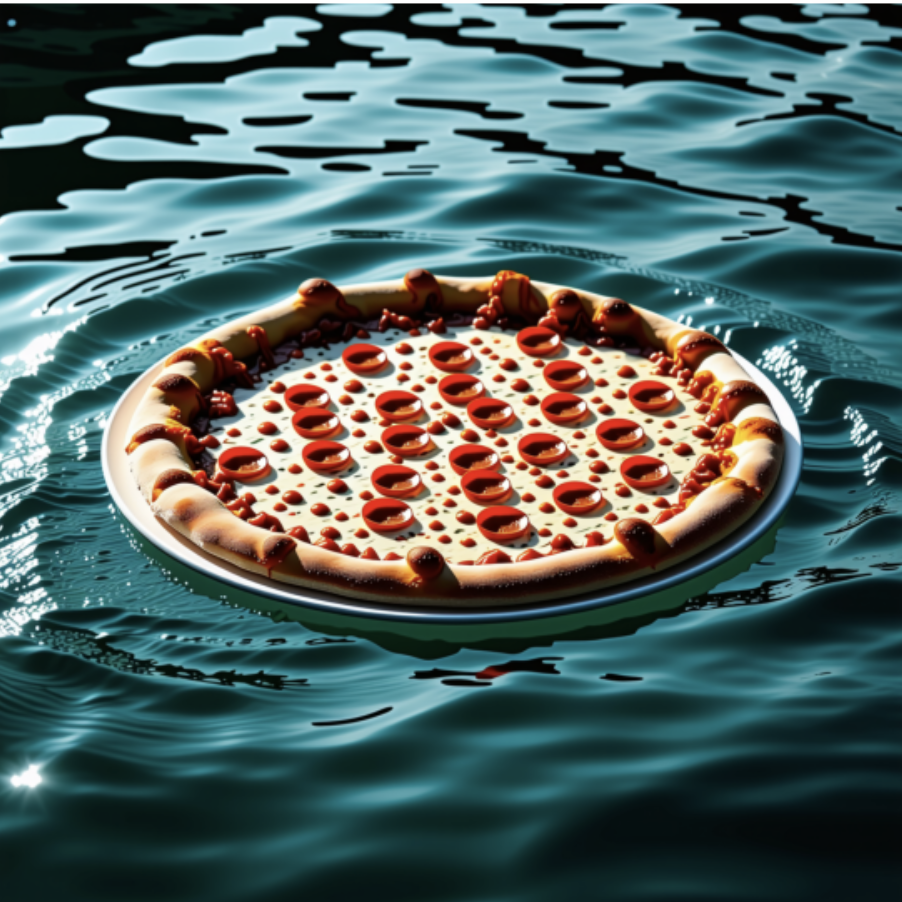
\includegraphics[width=0.19\textwidth]{plots/pizza.png}}
\subfigure[``A chessboard carved into stone.'']{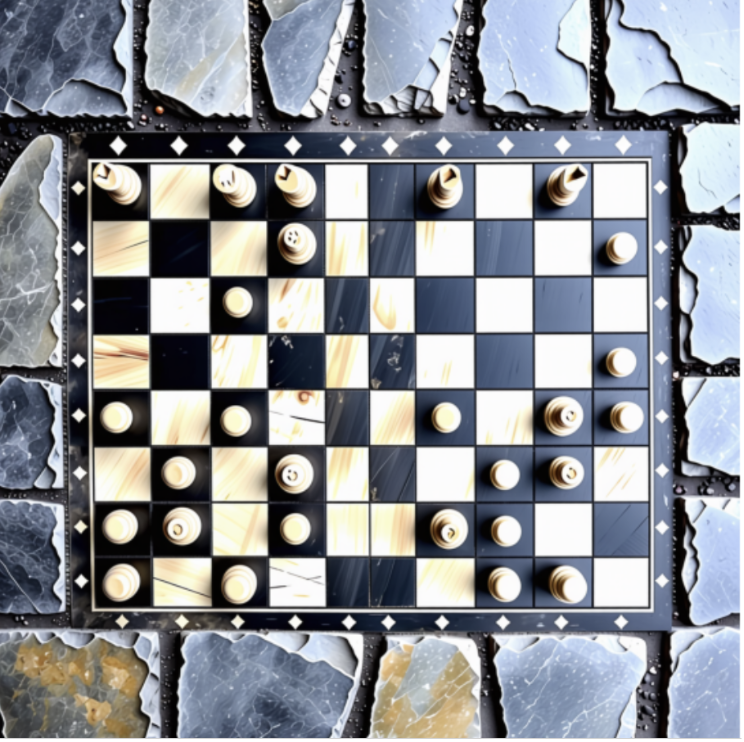
\includegraphics[width=0.19\textwidth]{plots/chessboard.png}}
\subfigure[``A person sketching a skyline on rooftop.'']{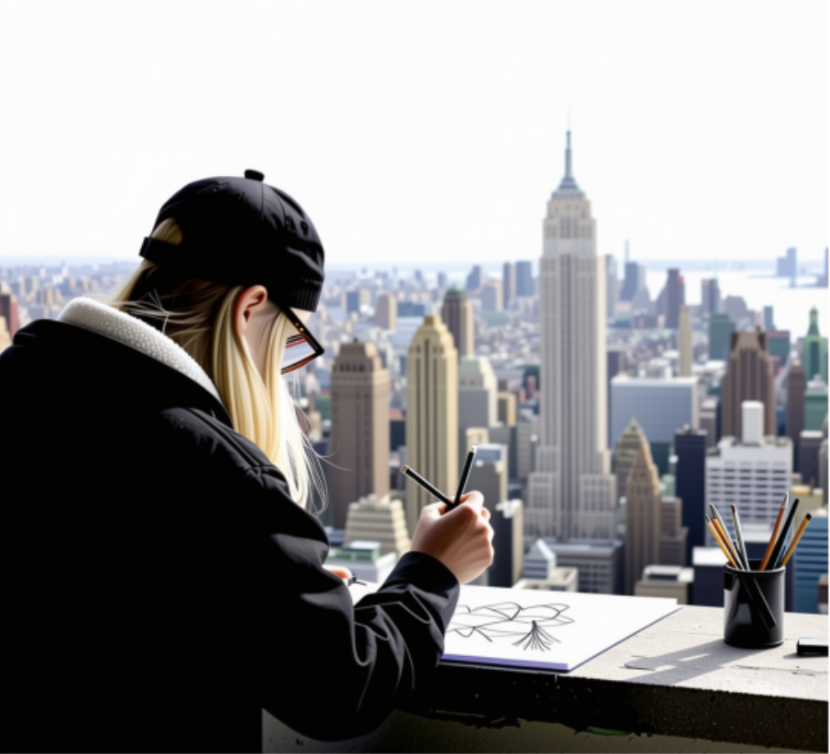
\includegraphics[width=0.19\textwidth]{plots/person.png}}
\subfigure[``A mirror reflecting only half of a person’s face.'']{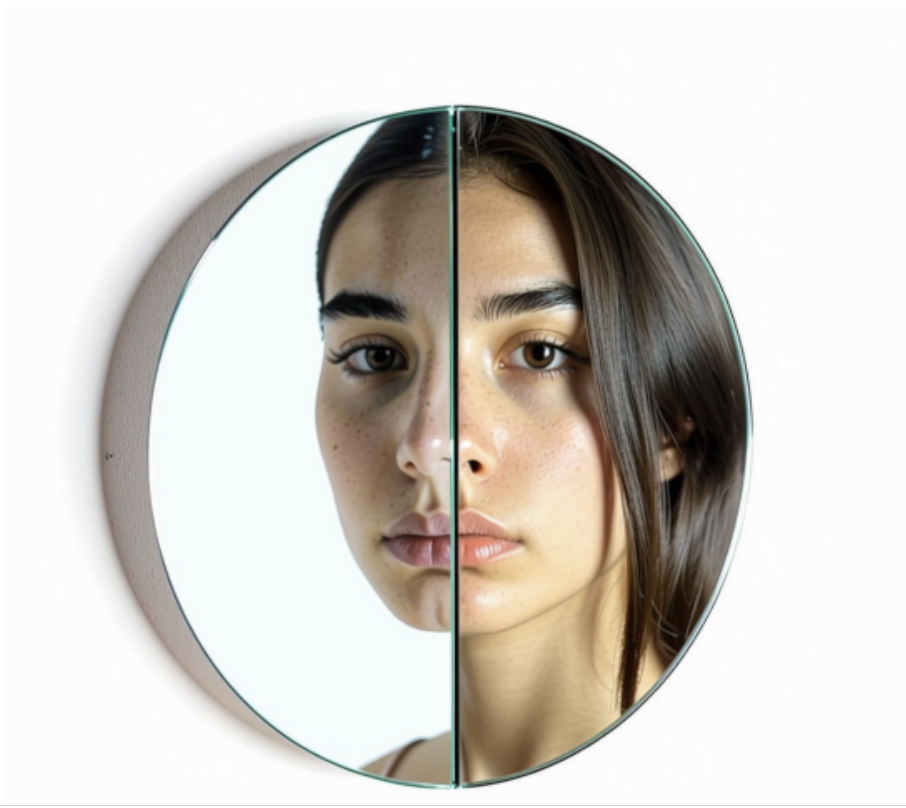
\includegraphics[width=0.19\textwidth]{plots/reflection.png}}
\subfigure[``A baby cow drinking milk from mother cow’s udder.'']{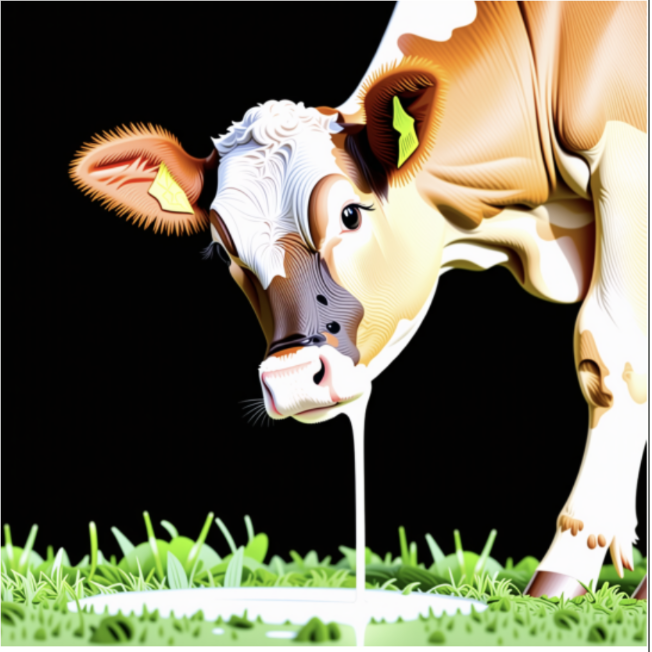
\includegraphics[width=0.19\textwidth]{plots/babycow.png}}
\caption{Notable failure modes discovered during the unconstrained exploration phase.}
\label{fig:comparison}
\end{center}
\vskip -0.2in
\end{figure*}

\subsection{Quantitative Analysis of Text Encoder Weights}
Analysis of the surgical replacement revealed significant statistical shifts within the model's embedding space. The weights of the RedCaps and CogVLM text encoders demonstrated variances of $1.395 \times 10^{-3}$ and $2.102 \times 10^{-3}$ compared to the original CLIP-L encoder, respectively. This confirmed the successful integration and functional divergence of the replacement text encoders within our pipeline. 

Furthermore, we performed a layer-by-layer weight divergence analysis between the original CLIP-L and the custom CLIC variants. Frobenius norms across the 12 transformer layers showed a consistently increasing trend from layer 0 to layer 11, with layer 11 exhibiting the largest total weight magnitude in both variants. Within the attention mechanisms, all projection matrices (Query, Key, Value, and Output) showed elevated norms in CogVLM relative to RedCaps, with Key projections (1.21$\times$ higher) and Value projections (1.22$\times$ higher) exhibiting the most pronounced differences. These elevations in attention projections suggest that the CogVLM variant may employ more fine-grained token relationships compared to the standard model. More detailed values across the layers of these weight differences is provided in Appendix \ref{sec:weights}.

\subsection{Comparative Model Behavior and Manual Observations}
Manual validation of 10 to 20 images per concept revealed distinctly different behavioral patterns between the standard baseline and the custom models.

\subsubsection{Baseline SD3.5}
From our investigation, we identified the following persistent limitations in the baseline model, as visualized in \cref{fig:sd_1}:
\begin{enumerate}
    \item \textbf{Positional Inversion and Order Bias:} The baseline performs poorly on the relation ``above,'' but fails significantly more often on ``below,'' as it frequently defaults to placing the first-mentioned object in the prompt above the second.
    \item \textbf{Lack of Scene Diversity:} The model is largely unable to generate counter-intuitive scenes rarely found in natural training datasets, such as a ``ball above book'' or a ``bench above cow''.
    \item \textbf{Directional Disparity:} While the model demonstrates adequate performance for ``to the left of'', it suffers a notable performance degradation when processing the inverse relation, ``to the right of''.
    \item \textbf{Inverse Spatial Logic:} For spatial prepositions like ``over'' and ``under'', the model frequently generates objects exhibiting the exact inverse of the requested spatial relationship.
\end{enumerate}

\begin{figure*}[t]
\vskip 0.2in
\begin{center}
\subfigure[``A photo of a giraffe below a hair drier.'']{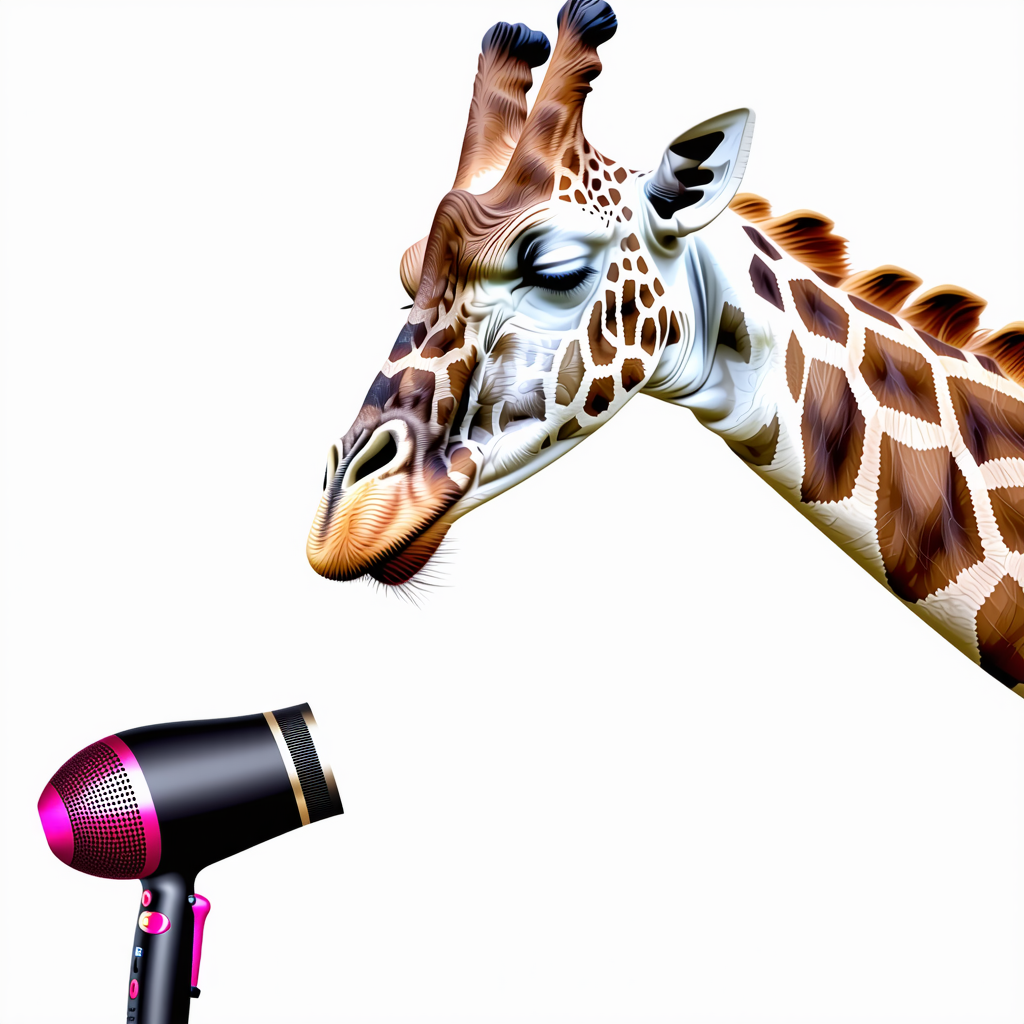
\includegraphics[width=0.19\textwidth]{plots/sd_below_giraffe_hair_drier_rank01_tidx0.png}}
\subfigure[``A photo of a bench above a cow.'']{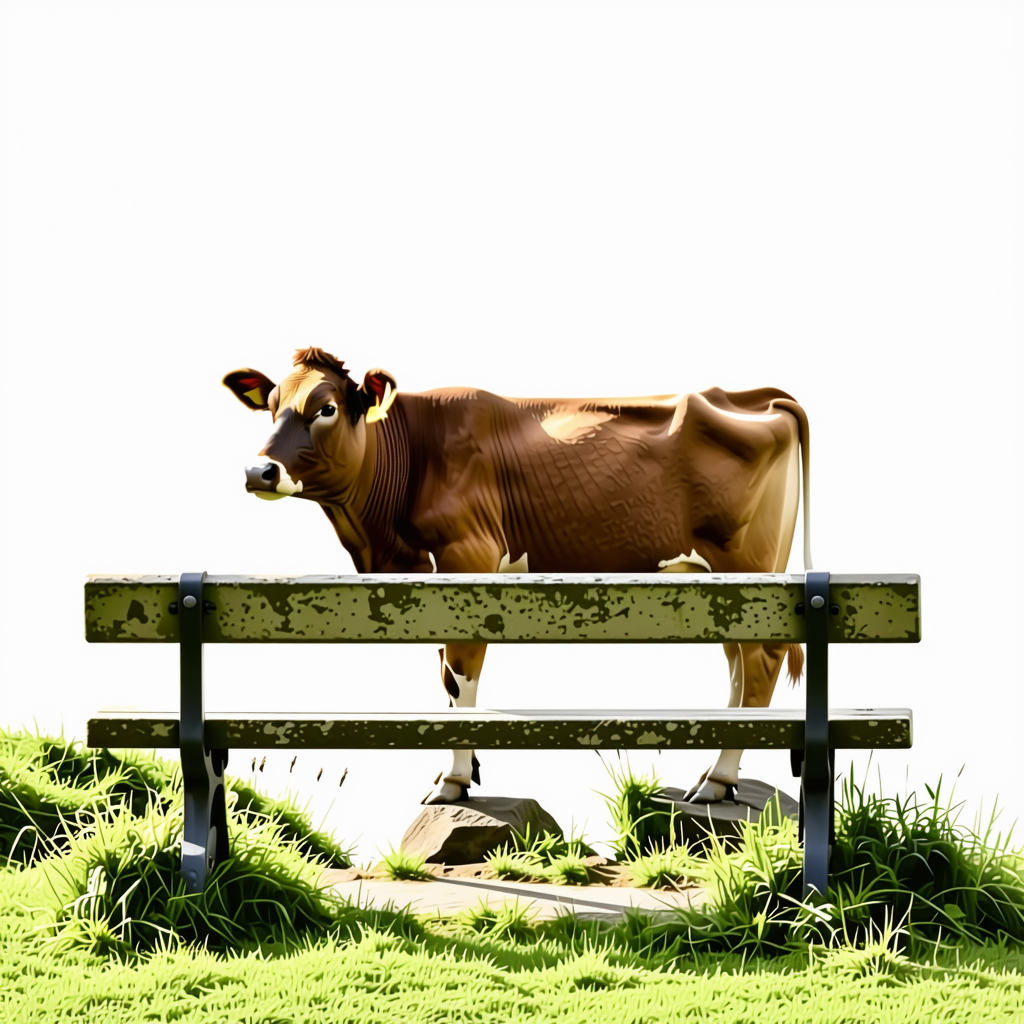
\includegraphics[width=0.19\textwidth]{plots/sd_above_bench_cow_rank04_tidx4.png}}
\subfigure[``A photo of a book above a sports ball.'']{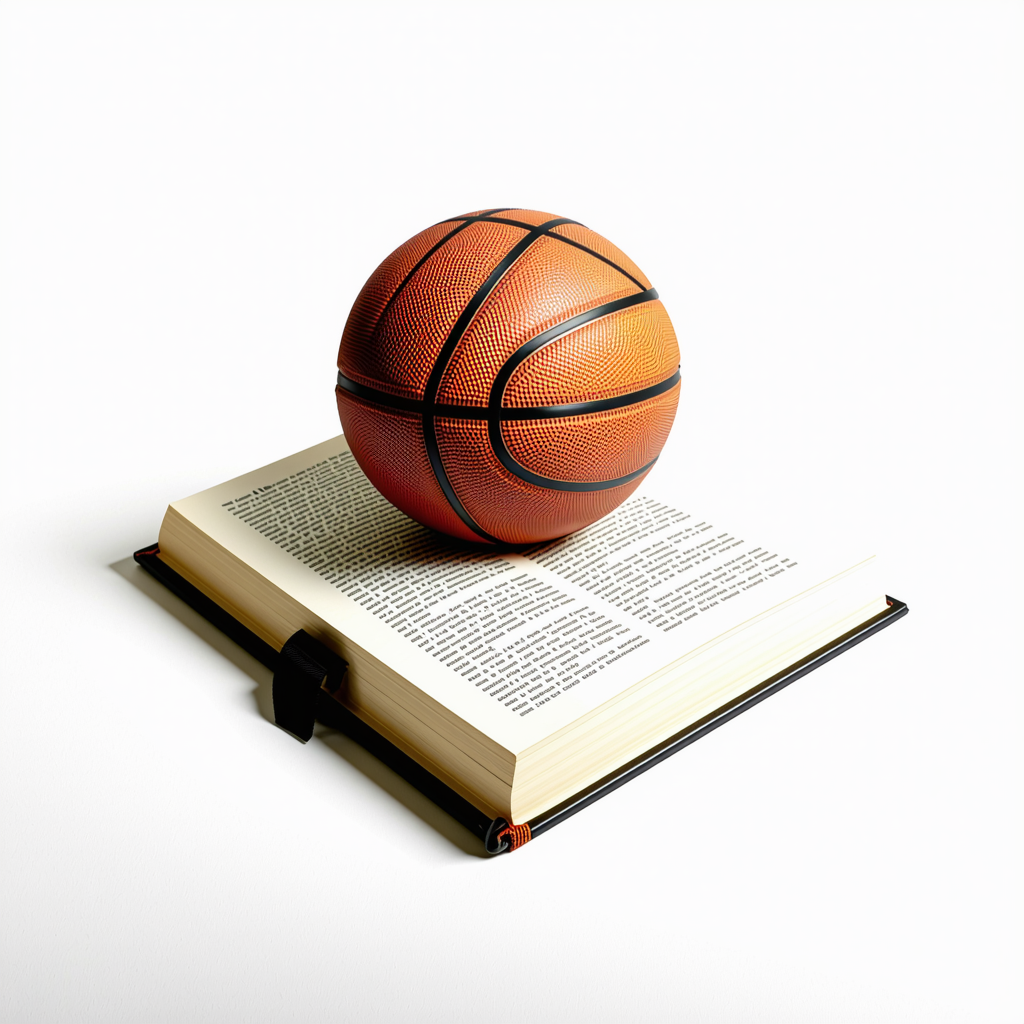
\includegraphics[width=0.19\textwidth]{plots/sd_above_book_sports_ball_rank03_tidx3.png}}
\subfigure[``A photo of a toilet to the left of a potted plant.'']{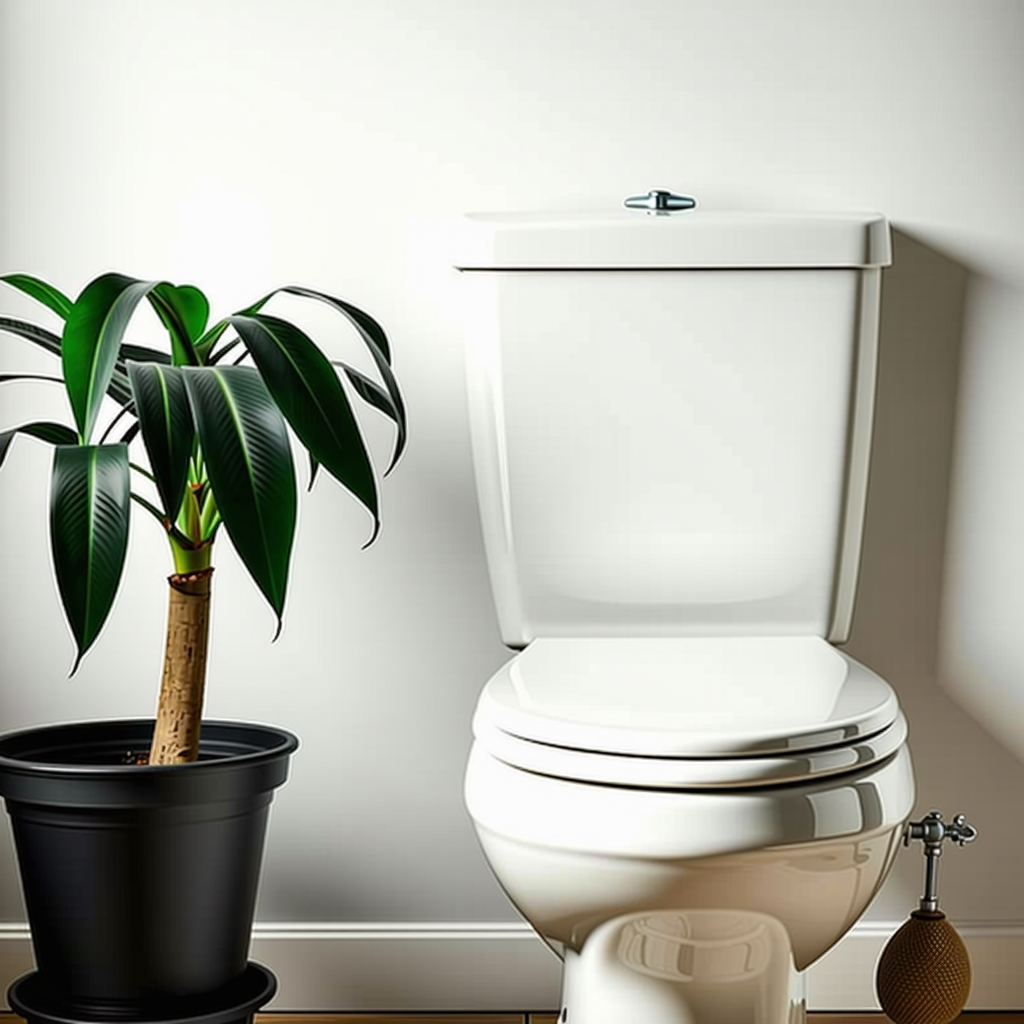
\includegraphics[width=0.19\textwidth]{plots/sd_to_the_left_of_toilet_potted_plant_rank06_tidx6.png}}
\subfigure[``A photo of a toilet to the right of a potted plant.'']{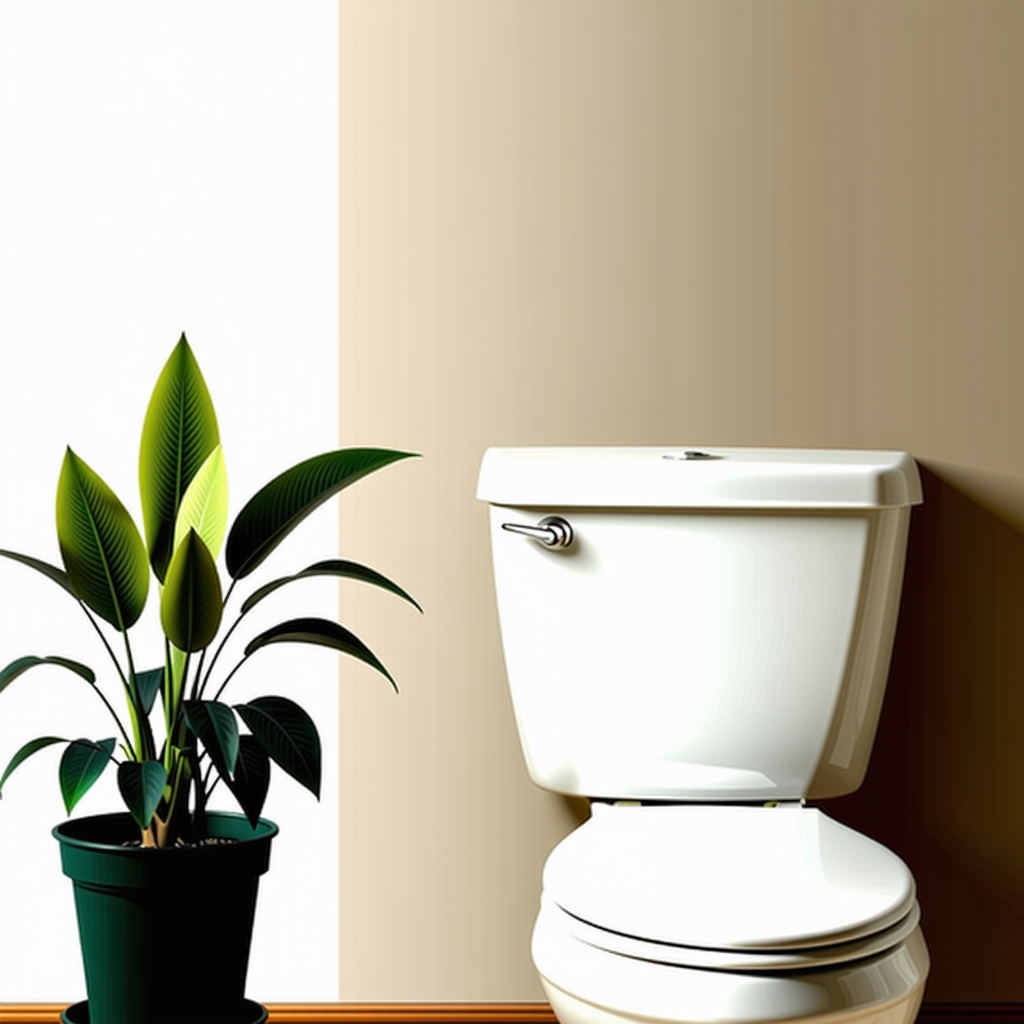
\includegraphics[width=0.19\textwidth]{plots/sd_to_the_right_of_toilet_potted_plant_rank06_tidx6.png}}
\caption{Standard SD3.5 outputs demonstrating spatial failure modes.}
\label{fig:sd_1}
\end{center}
\vskip -0.2in
\end{figure*}

\subsubsection{CLIC RedCaps and CogVLM}
Compared to Standard SD3.5, we observed the following improvements and anomalies, with examples shown in \cref{fig:clic}:
\begin{enumerate}
    \item \textbf{Improved Verticality and Containment:} RedCaps significantly outperforms the baseline in vertical reasoning and containment tasks (e.g., ``under'', ``over'', ``between''), although a minor fraction of images still exhibit generation errors.
    \item \textbf{Reduction in Ambiguity:} Both custom variants produced markedly fewer ambiguous or entirely fused images compared to the standard model.
    \item \textbf{CogVLM Performance Anomalies:} CogVLM behaves similarly to RedCaps overall but surprisingly performs worse on the phrases ``to the right of'' and ``between'' compared to RedCaps, despite still exceeding the baseline's performance. In certain edge cases, it replicates the exact spatial failures seen in Standard SD3.5.
\end{enumerate}

\begin{figure*}[t]
\vskip 0.2in
\begin{center}
\subfigure[``A photo of a giraffe below a hair drier.'']{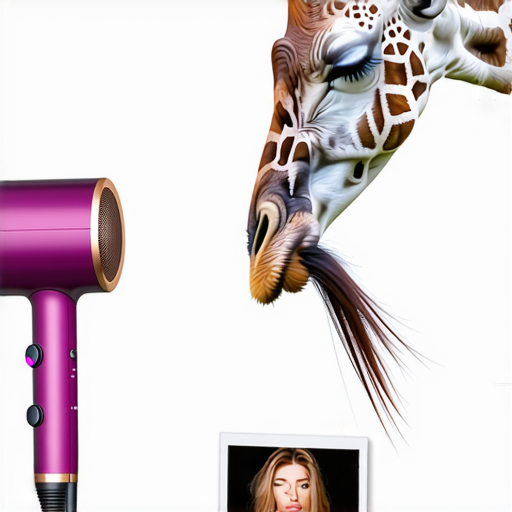
\includegraphics[width=0.19\textwidth]{plots/clic_below_giraffe_hair_drier_rank01_tidx0.png}}
\subfigure[``A photo of a bench above a cow'']{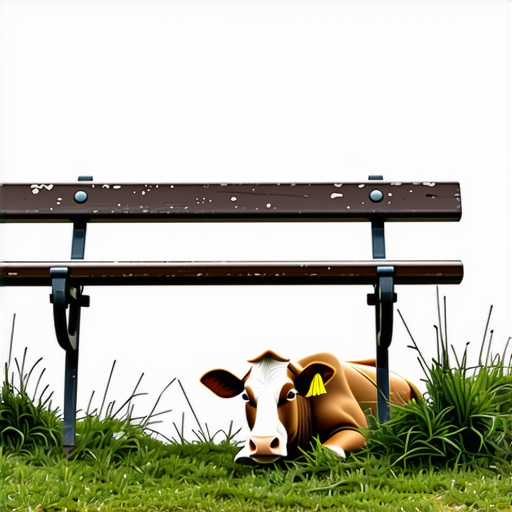
\includegraphics[width=0.19\textwidth]{plots/clic_above_bench_cow_rank04_tidx3.png}}
\subfigure[``A photo of a book above a sports ball.'']{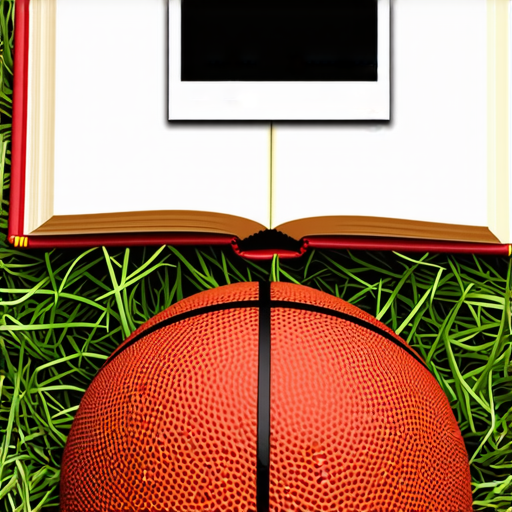
\includegraphics[width=0.19\textwidth]{plots/clic_above_book_sports_ball_rank03_tidx2.png}}
\subfigure[``A photo of a toilet to the left of a potted plant.'']{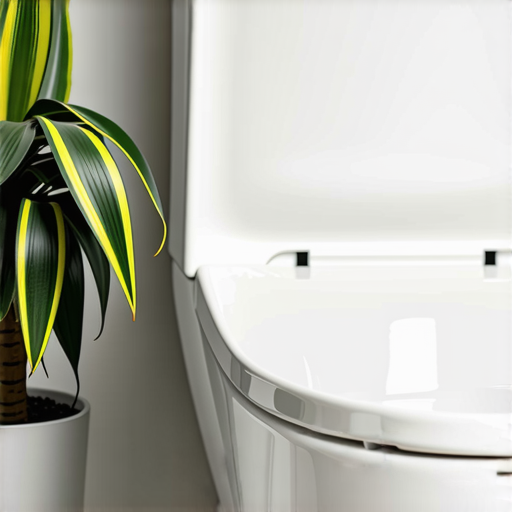
\includegraphics[width=0.19\textwidth]{plots/clic_to_the_left_of_toilet_potted_plant_rank06_tidx5.png}}
\subfigure[``A photo of a toilet to the right of a potted plant.'']{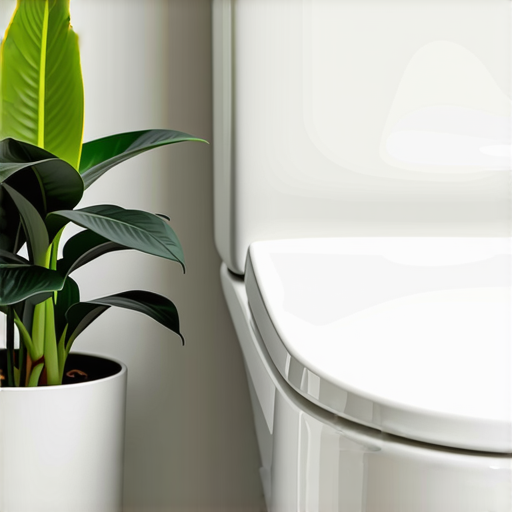
\includegraphics[width=0.19\textwidth]{plots/clic_to_the_right_of_toilet_potted_plant_rank06_tidx5.png}}

\subfigure[``A photo of a giraffe below a hair drier.'']{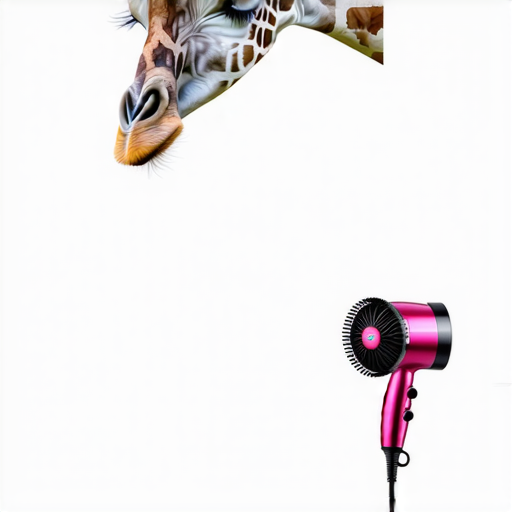
\includegraphics[width=0.19\textwidth]{plots/cogvlm_above_giraffe_hair_drier_rank01_tidx0.png}}
\subfigure[``A photo of a bench above a cow'']{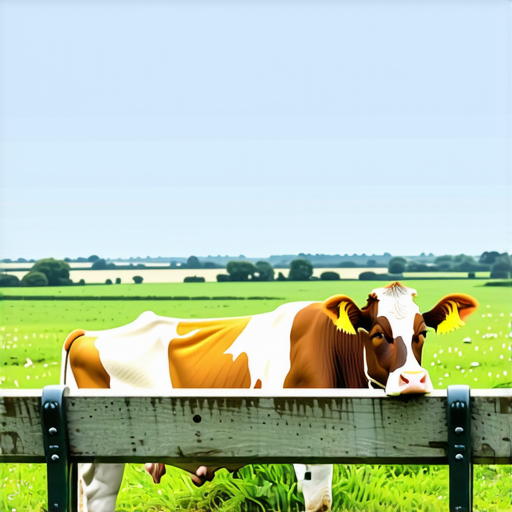
\includegraphics[width=0.19\textwidth]{plots/cogvlm_below_bench_cow_rank04_tidx3.png}}
\subfigure[``A photo of a book above a sports ball.'']{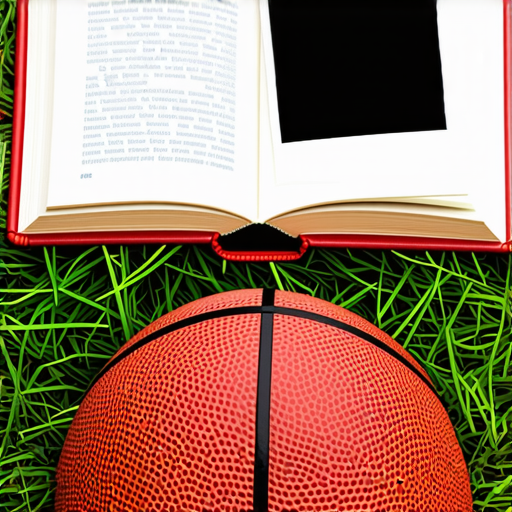
\includegraphics[width=0.19\textwidth]{plots/cogvlm_above_book_sports_ball_rank03_tidx2.png}}
\subfigure[``A photo of a toilet to the left of a potted plant.'']{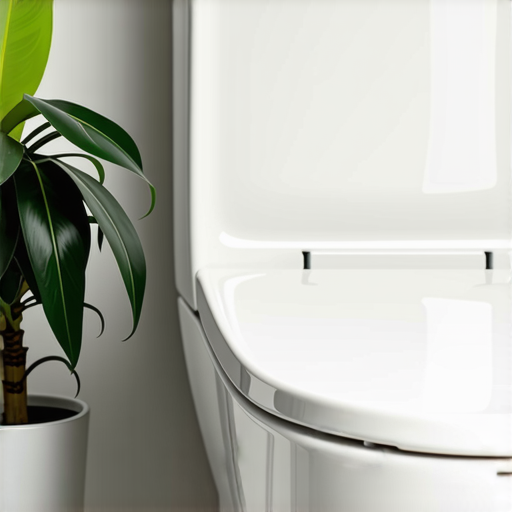
\includegraphics[width=0.19\textwidth]{plots/cogvlm_to_the_left_of_toilet_potted_plant_rank06_tidx5.png}}
\subfigure[``A photo of a toilet to the right of a potted plant.'']{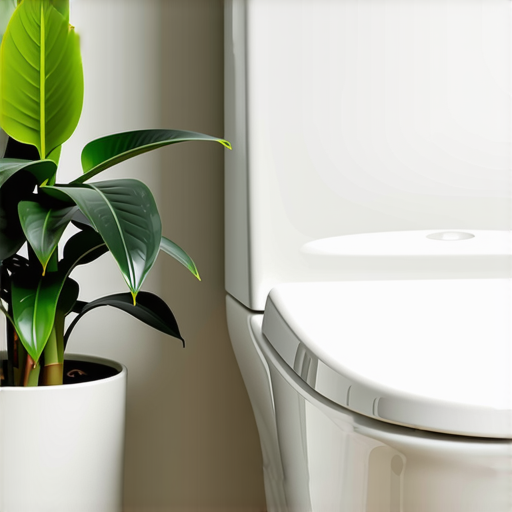
\includegraphics[width=0.19\textwidth]{plots/cogvlm_to_the_right_of_toilet_potted_plant_rank06_tidx5.png}}
\caption{RedCaps CLIC (top row) and CogVLM CLIC (bottom row) variant outputs.}
\label{fig:clic}
\end{center}
\vskip -0.2in
\end{figure*}

\begin{table}[ht]
\caption{Manual annotation results across the different SD3.5 variants, formatted as (Ambiguous, Incorrect, Correct). The number of manually checked images is listed in parentheses next to the phrase.}
\label{tab:manual}
\begin{center}
\begin{small}
\begin{tabular}{lccc}
\toprule
\textbf{Phrase} & \textbf{Standard} & \textbf{RedCaps} & \textbf{CogVLM} \\
\midrule
above (20) & (4,7,9) & (1,5,14) & (1,6,13) \\
below (20) & (4,8,8) & (1,12,7) & (0,9,11) \\
to the left of (20) & (4,5,11) & (0,9,11) & (0,8,12) \\
to the right of (20) & (1,17,2) & (0,9,11) & (0,11,9) \\
between (20) & (0,7,13) & (3,2,15) & (0,5,15) \\
behind (10) & (0,6,4) & (1,7,2) & (1,7,2) \\
closeby (10) & - & (0,1,9) & (0,1,9) \\
far from (10) & - & (0,7,3) & (0,6,4) \\
in front of (10) & (0,4,6) & (0,4,6) & (0,3,7) \\
without (10) & (0,7,3) & (0,6,4) & (1,5,4) \\
\bottomrule
\end{tabular}
\end{small}
\end{center}
\end{table}

\subsection{Quantitative Benchmark Results}
Following the pilot, we utilized a standardized taxonomy derived from the Self-Bench classes to evaluate over 1,600 generated prompts. Final accuracy was determined through automated Qwen3-VL-30B scoring, cross-referenced against our manual annotations. The comprehensive results are summarized in Table \ref{tab:accuracy}.

% \begin{table}[ht]
% \caption{Comparative accuracy across SD3.5 model variants (measured in percentage).}
% \label{tab:accuracy}
% \begin{center}
% \begin{small}
% \begin{tabular}{lccc}
% \toprule
% \textbf{Phrase} & \textbf{Standard} & \textbf{RedCaps} & \textbf{CogVLM} \\
% \midrule
% above & 72 & 90 & 95 \\
% below & 67 & 75 & 80 \\
% to the left of & 80 & 85 & 85 \\
% to the right of & 86 & 70 & 95 \\
% between & 76 & 50 & 55 \\
% behind & 65 & 60 & 60 \\
% closeby & - & 90 & 80 \\
% far from & - & 40 & 40 \\
% in front of & 60 & 70 & 70 \\
% on top of & 60 & 67 & 40 \\
% under & - & 60 & 30 \\
% over & 80 & 40 & 40 \\
% without & 80 & 50 & 50 \\
% \bottomrule
% \end{tabular}
% \end{small}
% \end{center}
% \end{table}

\begin{table}[ht]
\caption{Comparative accuracy across SD3.5 model variants using Majority-Voted VLM Scoring.}
\label{tab:accuracy}
\begin{center}
\begin{small}
\begin{tabular}{lccc}
\toprule
\textbf{Phrase} & \textbf{Standard SD3.5} & \textbf{RedCaps SD} & \textbf{CogVLM SD} \\
\midrule
above           & 72.73 & 85.00 & 90.00 \\
below           & 70.00 & 75.00 & 90.00 \\
to the left of  & 78.79 & 80.00 & 75.00 \\
to the right of & 84.85 & 65.00 & 80.00 \\
between         & 68.00 & -     & 55.00 \\
behind          & 63.16 & 60.00 & 60.00 \\
in front of     & 68.42 & 50.00 & 70.00 \\
on top of       & 33.33 & 30.00 & 20.00 \\
over            & 70.00 & 40.00 & 40.00 \\
under           & 40.00 & 40.00 & 30.00 \\
without         & 70.00 & 30.00 & 30.00 \\
\bottomrule
\end{tabular}
\end{small}
\end{center}
\end{table}


\subsection{Automated Evaluator Validation}
\subsubsection{LLaVA}
Our initial automated evaluation across core spatial phrases (such as ``above'', ``below'', ``to the left of'', and ``to the right of'') revealed that LLaVA yielded significant inconsistencies, achieving an overall accuracy of just 56.4\% (F1: 0.26). Specifically, on the phrase ``above'', LLaVA achieved a mere 43.18\% accuracy. Deeming this performance insufficient for reliable benchmarking, we pivoted to Qwen3-VL. This adjustment resulted in substantial improvements: our direct Qwen query approach achieved 73.48\% overall accuracy (F1: 0.62), while the expert reasoning-based Qwen approach reached a comparable 71.46\% accuracy (F1: 0.62).

\subsubsection{Qwen3-VL-30B}
We carefully measured the agreement between the Qwen3-VL-30B predictions and human evaluation. Table \ref{tab:redcaps_cm} presents a sample confusion matrix for the RedCaps SD variant (Phrase: ``Above'', $n=20$), demonstrating high evaluator reliability. Table \ref{tab:vlm_agreement} illustrates the overall agreement between manual labels and Qwen3-VL accuracies across different relational phrases.

\begin{table}[ht]
\caption{Sample Confusion Matrix demonstrating the high alignment (+80\% match) for the RedCaps model evaluating the ``above'' phrase utilizing the ``expert reasoning'' prompt strategy.}
\label{tab:redcaps_cm}
\begin{center}
\begin{small}
\begin{tabular}{lccc}
\toprule
 & \textbf{QWEN Yes} & \textbf{QWEN No} & \textbf{QWEN Amb} \\
\midrule
\textbf{Manual Yes} & 15 & 2 & 0 \\
\textbf{Manual No} & 0 & 3 & 0 \\
\textbf{Manual Amb} & 0 & 0 & 0 \\
\bottomrule
\end{tabular}
\end{small}
\end{center}
\end{table}

\begin{table*}[ht]
\caption{Qwen3-VL Agreement with Manual Annotations}
\label{tab:vlm_agreement}
\begin{center}
\begin{small}
\begin{tabular}{lccc}
\toprule
\textbf{Agreement Level} & \textbf{Standard SD3.5} & \textbf{RedCaps SD} & \textbf{CogVLM SD} \\
\midrule
\textbf{High Match (+80\%)} & right of, over, without & above, left, closeby & above, below, right of \\
\textbf{Decent (70-79\%)}    & above, left, between    & below, in front of    & in front of \\
\textbf{Poor Match (<70\%)}  & below, behind, on top   & right of, between, under & between, behind, far from \\
\bottomrule
\end{tabular}
\end{small}
\end{center}
\end{table*}

\begin{figure}[ht]
\vskip 0.2in
\begin{center}
\centerline{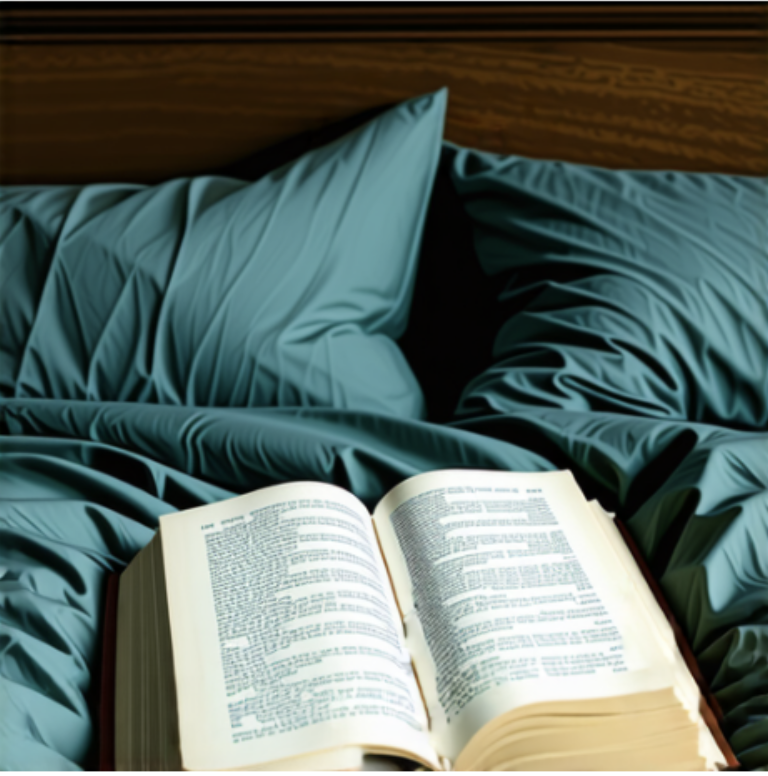
\includegraphics[width=0.5\columnwidth]{plots/clic - bed under book.png}}
\caption{An example of a Qwen3-VL failure mode where the model correctly identifies the objects and their relative physical positions but ultimately formulates an incorrect spatial conclusion.}
\label{fig:qwen-confusion}
\end{center}
\vskip -0.2in
\end{figure}

\subsubsection{VLM Logic and Reasoning Patterns}
Our deeper analysis of Qwen3-VL's internal reasoning traces identified critical failure bottlenecks in the evaluation pipeline. The VLM often reasons correctly about the visual elements but concludes with the incorrect logical answer. For example, regarding the image referenced in \cref{fig:qwen-confusion}, generated by the prompt ``A photo of a bed under a book'', Qwen3-VL correctly identifies both objects and describes their relative positions accurately: 

\textit{``1. The bed is identified as the large surface covered with teal bedding, including sheets and pillows, located in the lower and middle portions of the image... 2. The book is an open book with visible text, resting on top of the bed... 3. The book is physically located on top of the bed, not above it in a vertical sense. Therefore, the bed is not under the book in a spatial sense; rather, the book is on the bed. Conclusion: No.''} 

Despite this accurate breakdown, it ultimately concludes that the bed is \textit{not} under the book: a clear failure in spatial reasoning logic. This contradictory pattern was observed across multiple phrases. Furthermore, similar to the diffusion models themselves, the VLM evaluator frequently conflates ``left'' and ``right''. For the phrase ``in front of'', the VLM often rigidly expects direct physical occlusion, whereas our manual annotation accepted lateral foreground positioning. 

Additionally, during inverse prompting modes, the VLM frequently produced excessively verbose reasoning outputs. When the final answer was cut off due to token limits, this resulted in an automatic ``Ambiguous'' label across all models, though this specific failure occurred most frequently when evaluating the standard SD outputs.

\subsection{Image Fidelity (FID) Scores}
To ensure that improving compositional alignment did not degrade overall image quality, FID scores were calculated against 5,000 COCO validation images. As shown in Table \ref{tab:fid}, the custom text encoders maintained parity with and even marginally outperformed the standard model's generative quality, likely due to more precise feature alignment during the denoising process.

\begin{table}[ht]
\caption{FID Scores Against COCO Ground-Truth Validation Set}
\label{tab:fid}
\begin{center}
\begin{tabular}{lcc}
\toprule
\textbf{Model} & \textbf{FID Score}  \\
\midrule
Standard SD3.5  & 60.60 \\
CLIC RedCaps    & 57.92 \\
CogVLM Custom   & 57.86 \\
\bottomrule
\end{tabular}
\end{center}
\end{table}